\documentclass{article}

\usepackage{amsfonts}
\usepackage{amsmath}
% \usepackage{svg} %For including svgs
% \svgpath{{../assets/}}
\usepackage{graphicx}
\graphicspath{ {../assets/} }
\usepackage[margin=1in]{geometry} %Change margins
\usepackage{hyperref} %For hyperlinks in table of contents and other
\usepackage{float} %For using H in figure
\usepackage{subcaption} %For subfigures
\usepackage{booktabs} %For tables
\usepackage{multirow} %For tables

%\usepackage[charsperline=120]{jlcode} %For Julia Code Listing https://github.com/wg030/jlcode

\addtolength{\jot}{1em} %https://tex.stackexchange.com/questions/14679/amsmath-align-environment-row-spacing

\title{Optimization Assignment 3\\Linear Programs and Applications}
\date{Winter 2021}
\author{Kim Paolo Laberinto (7771083)}

\begin{document}
    \maketitle
    \newpage

    \tableofcontents
    \newpage


    \section{Q1. Linear Programming Applied to Diet Optimizaton}

    \subsection{Problem Set-up}

    In the assignment, a word problem was given in which a diet had to be constructed such that it minimized the total calorie content, while also still meeting the minimum daily nutriential requirements given.

    In this section the word problem will be formulated into linear program consisting of the following elements.
    \begin{itemize}
        \item Variables
        \item Objective Function
        \item Constraints
    \end{itemize}

    \subsubsection{Variables}

    \subsubsection{Objective Function}

    \subsubsection{Constraints}

    \subsection{Solution using Julia}

    The linear program was solved using JuMP.jl from the Julia ecosystem, yielding the following solution.

    % Solution

    \subsection{Solution using Matlab}

    The linear program was solved using Matlab, yielding the following solution.

    % Solution

    \subsection{Observations}

    There are several observations to make from these solutions.

    %Observations
    \begin{itemize}
        \item 
    \end{itemize}

    \subsection{Follow-up Question and Solution - Doubling Calories in Bran Muffins}

    A follow up question in the assignment was to determine what happens to the diet if the calories in the muffins are increased by a factor of 2.

    Using this new calorie content for the bran muffins yields the following solution.

    % Solution

    There are several observations to make from this new solution:

    %Observations
    \begin{itemize}
        \item 
    \end{itemize}


    \section{Q2. Example of Conversion to Standard Form}

    \section{Q3. Example of Graphically Solving a Linear Program}

    \begin{figure}[H]
        \centering
        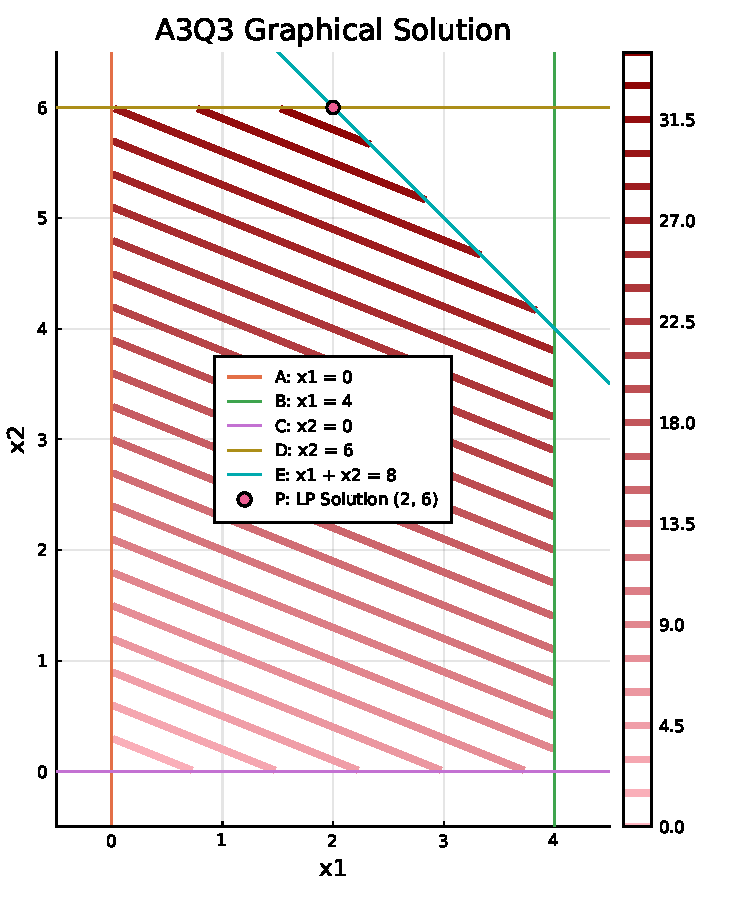
\includegraphics[width=0.5\linewidth]{A3Q3_Plot.pdf}
        \caption{Graphical Solution to A3Q3 question, showing feasible region, objective contours, and solution.}
        \label{fig:A3Q3_GraphicalSolution}
    \end{figure}

    \section{Q4. Textbook Questions}

    \subsection{12.9}

    \subsection{12.15}

    \subsection{12.21}

    \subsection{12.22}


    \newpage
    \appendix

    \section{Source Code}

\end{document}